\documentclass[11pt,letterpaper]{article}
\usepackage[lmargin=1in,rmargin=1in,bmargin=1in,tmargin=1in]{geometry}
\usepackage{style}

\setlength{\parindent}{0ex}

\usepackage{polynom}

% -------------------
% Content
% -------------------
\begin{document}

% Title
\begin{center} {\bfseries \LARGE MATH 142 --- Learning Outcomes --- Fall 2025} \end{center}

Here are some of the learning outcomes for each lecture. That is, after lecture, the homework, and studying, what students should know from each lecture. Though this list is not necessarily \textit{completely} comprehensive, the most important ideas/concepts are contained in each list. Students should be sure to feel comfortable with each bullet point before an exam. These learning goals are broken down by class date---with the class topic given. The classes are given in reverse-chronological order for ease of access to the most recent class. You may also click any of the hyperlinks below to jump to that date. 

\begin{itemize}
\item \hyperref[10-14]{10/14, Tuesday: Alternating Series Test \& Conditional Convergence}
\item \hyperref[10-07]{10/07, Thursday: Direct Comparison Test}
\item \hyperref[10-02]{10/02, Thursday: Limit Comparison Test}
\item \hyperref[09-30]{09/30, Tuesday: More Series \& Integral Test}
\item \hyperref[09-25]{09/25, Thursday: Sequences \& Series}
\item \hyperref[09-18]{09/18, Thursday: Arclength \& Surface Area}
\item \hyperref[09-16]{09/16, Tuesday: Improper Integrals}
\item \hyperref[09-11]{09/11, Thursday: Integration Review}
\item \hyperref[09-09]{09/09, Tuesday: Partial Fractions}
\item \hyperref[09-04]{09/04, Thursday: Partial Fractions}
\item \hyperref[09-02]{09/02, Tuesday: Trig. Substitution}
\item \hyperref[08-28]{08/28, Thursday: Trigonometric Integrals}
\item \hyperref[08-26]{08/26, Tuesday: Integration-by-Parts}
\item \hyperref[08-21]{08/21, Thursday: Integration-by-Parts}
\item \hyperref[08-19]{08/19, Tuesday: $u$-Substitution Review}
\end{itemize}

% 10/14, Tuesday: Alternating Series Test & Conditional Convergence
\newpage
\section*{10/14, Tuesday: Alternating Series Test \& Conditional Convergence\label{10-14}}

\begin{itemize}
\item Know that an alternating series is a series of the form $\ds\sum^\infty (-1)^n a_n$, where $\{ a_n \}$ is a sequence with $a_n > 0$. That is, an alternating series is a series whose terms alternate sign. 

\item Know that the Comparison Tests \textit{do not} apply to alternating series.

\item Be able to understand, state, and use the Alternating Series Test (AST): if $\ds\sum^\infty (-1)^n a_n$ is an alternating series with\dots
	\begin{itemize}
	\item $\ds\lim_{n \to \infty} a_n= 0$
	\item $\{ a_n \}$ is a decreasing sequence, i.e. $a_{n+1} \leq a_n$
	\end{itemize}
Then the series $\ds\sum^\infty (-1)^n a_n$ converges.

\item Know that the first part of the Alternating Series Test is simply the Divergence Test and that if in an alternating series $\ds\lim_{n \to \infty} a_n \neq 0$, then the series diverges by the Divergence Test. [Even though we only know $\ds\lim_{n \to \infty} a_n \neq 0$ and not necessarily $\ds\ds\lim_{n \to \infty} (-1)^n a_n \neq 0$. It is true that if $\ds\lim_{n \to \infty} a_n \neq 0$, then $\ds\lim_{n \to \infty} (-1)^n a_n \neq 0$, so that the Divergence Test will apply.]

\item Know that to show a sequence is decreasing, one often has to use derivatives, i.e. showing the derivative is always negative, or some type of `algebraic' trick. Although, we often will not bother to \textit{prove} that the sequence is (eventually) decreasing but instead rather simply assume/state it.

\item Know that if an $\{ a_n \}$ is not necessarily decreasing (so that the Alternating Series Test does not apply), this \textit{does not} mean that the alternating series diverges----it may converge or it may diverge. For example, the alternating series given by $\dfrac{1}{2^4} - \dfrac{1}{2^2} + \dfrac{1}{3^4} - \dfrac{1}{3^2} + \dfrac{1}{4^4} - \dfrac{1}{4^2} + \cdots$ has terms that tend to 0 but do not decrease, e.g. $\frac{1}{2^2} \not\leq \dfrac{1}{2^4}$. Yet, this series converges. On the other hand, the series given by $\dfrac{1}{\sqrt{2} - 1} - \dfrac{1}{\sqrt{2} + 1} + \dfrac{1}{\sqrt{3} - 1} - \dfrac{1}{\sqrt{3} + 1} + \cdots$ has terms that tend to 0 but do not decrease, e.g. the given terms are $\approx 2.41421, 0.414214, 1.36603, 0.366025, \ldots$. But this series does indeed diverge. 

\item Know that the Alternating Harmonic Series converges. In fact, $\ds\sum_{n=1}^\infty \dfrac{(-1)^{n+1}}{n}= \ln(2)$.

\item Know that while many alternating series have a power of $-1$, alternating series do not have to have this to be alternating---the term could be `hidden.' For example, the series $\ds\sum_{n=1}^\infty \dfrac{n \cos(\pi n)}{\ln(n + 1)}$ is alternating because the values of $\cos(\pi n)$ are either $+1$ or $-1$ depending on the value of $n$. Furthermore, just because a series has a power of $-1$ in the summand does not mean that the series alternates. For example, the series $\ds\sum_{n=1}^\infty \dfrac{(-1)^n}{(-2)^n}$ \textit{does not} alternate because $\ds\sum_{n=1}^\infty \dfrac{(-1)^n}{(-2)^n}= \sum_{n=1}^\infty \dfrac{(-1)^n}{(-1)^n 2^n}= \sum_{n=1}^\infty \dfrac{1}{2^n}= \sum_{n=1}^\infty \left( \dfrac{1}{2} \right)^n$, which does not alternate. 

\item Be able to know, state, and apply the Remainder Theorem for Alternating Series: if an alternating series $\ds\sum^\infty (-1)^n a_n$ converges, say to $S$, then the difference between $S$ and the sum of the first $n$ terms, $S_n$ (which is called the remainder, $R_n$) satisfies $|S_n - S|= |R_n| \leq |a_{n+1}|$. That is, the error between the actual sum of the series and the sum you get by adding the first $n$ terms is at most the magnitude of the next term you would have added/subtracted next. For instance, the series $\ds\sum_{n=1}^\infty \dfrac{(-1)^{n+1}}{n}$ converges by the Alternating Series Test (in fact, to $\ln(2)$). If we only add $1 - \frac{1}{2} + \frac{1}{3} - \frac{1}{4} + \frac{1}{5} - \frac{1}{6} + \frac{1}{7} \approx 0.759524$, then the error between this value and the actual sum of the series is \textit{at most} $\left| -\frac{1}{8} \right|= \frac{1}{8}= 0.125$. In fact, $|\ln(2) - 0.759524| \approx 0.0663766 < 0.125$.

\item Be able to use the Remainder Theorem for Alternating Series to find at most how many terms of a convergent alternating series one would need to add to be within a certain error of the actual sum of the series. For instance, we know the series $\ds\sum_{n=1}^\infty \dfrac{(-1)^n}{\sqrt{n}}$ converges by the Alternating Series Test. Suppose one wanted to find the sum of this series to two decimal places, i.e. with an error less than $\pm 0.01$. If we added the first $n$ terms, the magnitude of the next term would be $\frac{1}{\sqrt{n+1}}$. We know the error is at most this term. So, we could find an $n$ such that $\frac{1}{\sqrt{n+1}} < 0.01$. But then\dots
	\[
	\begin{gathered}
	\dfrac{1}{\sqrt{n+1}} < 0.01 \\[0.2cm]
	\dfrac{1}{\sqrt{n+1}} < \dfrac{1}{100} \\[0.2cm]
	\sqrt{n+1} > 100 \\[0.2cm]
	(\sqrt{n+1})^2 > 100^2 \\[0.2cm]
	n + 1 > 10000 \\[0.2cm]
	n > 9999
	\end{gathered}
	\]
Therefore, if we add at least the first $9,\!999+1= 10,\!000$ terms of the series (the $+1$ is because this is the next integer strictly bigger than $9,\!999$; if we had $n > 8,\!432.119$, we would have taken $n= 8,\!433$), we would approximate the actual sum to two decimal places. We may need less terms, but using this many guarantees it. 

\item Know that dropping/moving infinitely many parentheses is not necessarily a valid operation; that is, while moving finitely many parentheses is fine, e.g. $(1 + 3) - 4 + 6 + (5 - 1)= 1 + (3 - 4) + (6 + 5) - 1$, but something like $(1 - 1) + (1 - 1) + (1 - 1) + \cdots= 1 + (-1 + 1) + 1 + (-1 + 1) + \cdots$ is not necessarily (and often is not) correct. 

\item Know and be able to state the definition of absolute and conditional convergence: a series $\ds\sum a_n$ is absolutely convergent (or converges absolutely) if $\ds\sum |a_n|$ also converges. If $\ds\sum a_n$ converges but the series $\ds\sum |a_n|$ diverges, then we say that the series $\ds\sum a_n$ converges conditionally (or is conditionally convergent). 

\item Know that if the series $\ds\sum |a_n|$ converges, i.e. the series $\ds\sum a_n$ is absolutely convergent, then it must be that the series $\ds\sum a_n$ converges. In fact, if a series $\ds\sum a_n$ is absolutely convergent, then the series created by  \textit{any} rearrangement of its terms converges and also converges to the same sum. This is called the Riemann Rearrangement Theorem.

\item Know that if a series $\ds\sum a_n$ is conditionally convergent, i.e. $\ds\sum a_n$ converges but $\ds\sum |a_n|$ diverges, then there is a series that can be formed by rearranging the terms of the series $\ds\sum a_n$ that converges to \textit{any} real number, $-\infty$, $+\infty$, or diverges. This is called the Riemann Rearrangement Theorem.

\item Be able to determine whether a given series diverges, converges conditionally, or converges absolutely and be able to provide a full justification of the answer. 
\end{itemize}

% 10/07, Thursday: Limit Comparison Test
\newpage
\section*{10/07, Thursday: Direct Comparison Test\label{10-07}}

\begin{itemize}
\item Understand and be able to state the Direct Comparison Test: if $\{ a_n \}$ and $\{ b_n \}$ are sequences with $a_n, b_n > 0$ such that $\ds\sum^\infty a_n \leq \sum^\infty b_n$, then\dots
	\begin{itemize}
	\item If $\ds\sum^\infty a_n$ diverges, then $\ds\sum^\infty b_n$ diverges. 
	\item If $\ds\sum^\infty b_n$ converges, then $\ds\sum^\infty a_n$ converges.
	\end{itemize}

\item Understand and be able to articulate why the Direct Comparison Test works, i.e. be able to understand and explain why one series being larger/smaller than the other assures the others convergence/divergence. 

\item If a series is `like' a $p$-series, be able to determine which $p$-series it is `like' and use this information to predict whether the given series converges or diverges.

\item Understand that to make a fraction larger, one needs to make the numerator larger or the denominator smaller. To make a fraction smaller, one needs to make the numerator smaller or the denominator larger. 

\item Be able to use the Direct Comparison Test to prove that a given series converges or diverges, including cases where one needs to be `clever'.

\item Be able to use a `number line' analogy to help determine whether one needs to increase or decrease the summand to prove the convergence/divergence of the given series with the Direct Comparison Test. 

\item Understand when the Direct Comparison Test cannot be used and instead the Limit Comparison Test is needed. 

\item Know that the Direct Comparison Test cannot be used for alternating series. 
\end{itemize}

% 10/02, Thursday: Limit Comparison Test
\newpage
\section*{10/02, Thursday: Limit Comparison Test\label{10-02}}

\begin{itemize}
\item Understand and be able to state the Limit Comparison Test: if $\{ a_n \}$ and $\{ b_n \}$ are sequences with $a_n, b_n > 0$ such that $\ds\lim_{n \to \infty} \dfrac{a_n}{b_n}$ is finite and not 0, then $\ds\sum^\infty a_n$ and $\ds\sum^\infty b_n$ either both converge or both diverge. 

\item Understand and be able to articulate why the Limit Comparison Test works, i.e. be able to understand and explain why the limit being finite and nonzero means one series is `like' the other. 

\item If a series is `like' a $p$-series, be able to determine which $p$-series it is `like' and use this information to predict whether the given series converges or diverges.

\item Be able to use the Limit Comparison Test to prove that a given series converges or diverges. 

\item Know that the Limit Comparison Test cannot be used for alternating series. 
\end{itemize}

% 09/30, Tuesday: More Series & Integral Test
\newpage
\section*{09/30, Tuesday: More Series \& Integral Test\label{09-30}}

\begin{itemize}
\item Know that for now the focus of the course is determining whether a given series converges and diverges with a full justification. In special cases, if the series converges, then also finding its sum.
\item Know when the Divergence Test applies and when it does not apply.
\item Be able to use the Divergence Test to prove that a given series diverges.
\item Recall that the series $\ds\sum^\infty \dfrac{1}{n}$ is called the Harmonic series and that this series diverges. 
\item Be able to identify a $p$-series.
\item Be able to recognize a rational function as being `like' a $p$-series---even when it is not. For example, one should recognize that $\ds\sum^\infty \dfrac{n + 1}{n^3 - 5}$ is `like' the $p$-series $\ds\sum^\infty \dfrac{1}{n^2}$ because for `large' $n$, the summand $\dfrac{n + 1}{n^3 - 5}$ is `like' $\dfrac{n}{n^3}= \dfrac{1}{n^2}$.
\item Understand the difference between a series and the sequence making up the summand of a series and be able to use this language correctly in given contexts, i.e. the `no pronoun' rule.
\item Be able to recognize a geometric series and write it in the form $\ds\sum a r^n$. 
\item Be able to determine whether a geometric series converges or diverges and if the series converges find its sum.
\item Be able to write a real number with a finite or repeating decimal expansion as a fraction, especially using a geometric series. 
\item Be able to identify a Telescoping series. 
\item Be able to determine whether a Telescoping series converges or diverges and if the series converges to find its sum. 
\item Be able to state the Integral Test and know when it applies: if $\{a _n \}$ is a sequence of positive real numbers and $a_n= f(n)$, where $f(x)$ is a continuous, positive, and decreasing function, then $\ds\sum^\infty a_n$ converges if and only if $\ds\int^\infty f(x) \;dx$ converges; that is, either both the integral and series both converge or the integral and the series both diverge. 
\item Be able to articulate why the Integral Test is true through a graphical example. 
\item Be able to use the Integral Test to determine whether a given series converges or diverges.
\item Know that if the Integral Test determines that a given series converges that the integral and series \textit{do not} have to have the same value (and very likely do not). 
\end{itemize}

% 09/25, Thursday: Sequences \& Series
\newpage
\section*{09/25, Thursday: Sequences \& Series\label{09-25}}

\begin{itemize}
\item Know the definition of a sequence.
\item Be able to give examples of sequences, including some famous sequences.
\item Be able to compute terms of a sequence given its formula. 
\item Be able to determine a formula for a given sequence. 
\item Be able to compute terms of a recursive sequence. 
\item Be able to explain how an infinite series is defined (in terms of partial sums). 
\item Know that an infinite series converges if its partial sums converge and diverges otherwise.
\item Know that $\ds\sum_{n=1}^\infty \dfrac{1}{n}$ is called the Harmonic Series and diverges (to $\infty$).
\item Be able to state the Divergence Test ($n$th Term Test): if $\ds\lim_{n \to \infty} a_n \neq 0$, then $\ds\sum^\infty a_n$ diverges. 
\item Know when the Divergence Test applies and does not apply to an infinite series. 
\item Be able to use the Divergence Test to show that a series diverges.
\item Be able to give an example where the Divergence Test does not apply (because $\ds\lim_{n \to \infty} a_n= 0$) but the series diverges, e.g. $\ds\sum_{n=1}^\infty \dfrac{1}{n}$, and another where the series converges, e.g. $\ds\sum_{n=1}^\infty \dfrac{1}{n^2}$.
\item Know that a $p$-series is an infinite series of the form $\ds\sum^\infty \dfrac{1}{n^p}$. 
\item Be able to identify whether a given infinite series is a $p$-series or not. 
\item Know the $p$-series Test:
	\[
	\sum^\infty \dfrac{1}{n^p}= \begin{cases} \text{converges}, & p > 1 \\ \text{diverges (to } \infty \text{)}, & p \leq 1 \end{cases}
	\]
\item Be able to define and give examples of a geometric sequence---a sequence with a common multiple/ratio.
\item Be able to define and identify a geometric series---a series of the form $\ds\sum a r^n$. 
\item Know that the sum of a finite geometric series is given by\dots
	\[
	\sum_{k=0}^n a r^k= a \, \dfrac{1 - r^{n+1}}{1 - r}
	\]
\item Know the Geometric Series Test: if a geometric series has common ratio $r$ and $|r| < 1$, then the infinite series converges to $\frac{\text{first term}}{1 - r}$; otherwise, the series diverges. 
\item Be able to compute the sum of a finite geometric series. 
\item Be able to determine whether a given infinite geometric series converges or diverges and if it converges compute its sum. 
\end{itemize}

% 09/18, Thursday: Arclength \& Surface Area
\newpage
\section*{09/18, Thursday: Arclength \& Surface Area\label{09-18}}

\begin{itemize}
\item Be able to explain the idea of how the arclength formula is derived. 
\item Know that the arclength of the portion of the graph of $f(x)$ between $x= a$ and $x= b$ is\dots
	\[
	L= \int_a^b \sqrt{1 + \big( f'(x) \big)^2} \;dx
	\]
\item Be able to compute the arclength of a curve.
\item Be able to explain the idea of how the surface area formula is derived. 
\item Know that the surface area resulting from revolving the portion of the graph of $f(x)$ between $x= a$ and $x= b$ around the $x$-axis is\dots
	\[
	\text{SA}= 2\pi \int_a^b f(x) \sqrt{1 + \big( f'(x) \big)^2} \;dx
	\]
\item Know that the `$f(x)$' in the formula above is really a `radius' from the portion of the graph at $x$ to the axis of revolution---allowing one to alter the above formula for other situations. 
\item Be able to compute the surface area of a given surface. 
\end{itemize}

% 09/16, Tuesday: Improper Integrals
\newpage
\section*{09/16, Tuesday: Improper Integrals\label{09-16}}

\begin{itemize}
\item Know that an integral is improper if either of the limits are $\pm\infty$ or if the integrand is undefined at some value between the limits of integration.
\item Know how to properly write an improper integral using a limit. 
\item Know that an integral which is improper at both endpoints or at a value in-between the limits of integration must be broken into two integrals. 
\item Know that an improper integral converges if the limit of all the integral(s) making it up exist. Otherwise, the improper integral diverges. 
\item Be able to determine the value of an improper integral (if it converges). 
\item Know that\dots
	\[
	\int_1^\infty \dfrac{1}{x^p} \;dx= \begin{cases} \dfrac{1}{p - 1}, & p > 1 \\ \infty, & p \leq 1 \end{cases}
	\]
\end{itemize}

% 09/11, Thursday: Integration Review
\newpage
\section*{09/11, Thursday: Integration Review\label{09-11}}

\begin{itemize}
\item Be able to identify what method of integration a particular integral may require: Partial Fraction $\to$ Trig. Sub $\to$ Trigonometric $\to$ $u$-Sub (Shifting) $\to$ IBP (+ tabular \& looping) $\to$ Other (algebra, identities, `weird' $u$-sub, etc.)
\end{itemize}

% 09/09, Tuesday: Partial Fractions
\newpage
\section*{09/09, Tuesday: Partial Fractions\label{09-09}}

\begin{itemize}
\item Know what Heaviside's Method/Cover-Up Method (without modification) can find in a partial fraction decomposition (the term for the highest power of a linear term). For example, 
	\[
	\begin{aligned}
	\dfrac{\;\;\;\rule{1cm}{0.3pt}\;\;\;}{(x - 2)(x + 3)}&= \dfrac{\boxed{A}}{x - 2} + \dfrac{\boxed{B}}{x + 3} \\
	\dfrac{\;\;\;\rule{1cm}{0.3pt}\;\;\;}{x^2(x + 5)}&= \dfrac{A}{x} + \dfrac{\boxed{B}}{x^2} + \dfrac{\boxed{C}}{x + 5} \\
	\dfrac{\;\;\;\rule{1cm}{0.3pt}\;\;\;}{x(x^2 + 4)}&= \dfrac{\boxed{A}}{x} + \dfrac{Bx + C}{x^2 + 4} \\
	\dfrac{\;\;\;\rule{1cm}{0.3pt}\;\;\;}{x(x + 2)^2}&= \dfrac{\boxed{A}}{x} + \dfrac{B}{x + 2} + \dfrac{\boxed{C}}{(x + 2)^2}
	\end{aligned}
	\]
Heaviside's method (without modification) will only find the boxed coefficients above. Other work will be required to find the other terms. 

\item Be able to use Heaviside's method in a partial fractions integral, e.g. 
	\[
	\int \dfrac{x + 3}{(x - 1)(x + 2)} \;dx
	\]
	\[
	\dfrac{x + 3}{(x - 1)(x + 2)}= \dfrac{A}{x - 1} + \dfrac{B}{x + 2}
	\]
	\[
	A= \dfrac{1 + 3}{1 + 2}= \dfrac{4}{3} \qquad B= \dfrac{-2 + 3}{-2 - 1}= \dfrac{1}{-3}
	\]
	\[
	\int \dfrac{x + 3}{(x - 1)(x + 2)} \;dx= \int \dfrac{4/3}{x - 1} + \dfrac{-1/3}{x + 2} \;dx= \tfrac{4}{3} \ln|x - 1| - \tfrac{1}{3} \ln|x + 2| + K
	\]

\item Be able to complete a partial fractions integral when Heaviside's method fails to compute all terms. 

\item Know other `shortcut' methods for partial fractions, e.g. evaluating the expressions at various $x$-values. 
\end{itemize}

% 09/04, Thursday: Partial Fractions
\newpage
\section*{09/04, Thursday: Partial Fractions\label{09-04}}

\begin{itemize}
\item Be able to long divide polynomials, e.g.
	\[
	\polylongdiv{X^3+X^2-1}{X-1}
	\]

\item Recall that for a partial fraction decomposition, the degree of the numerator must be \textit{less than} the degree of the denominator.

\item Be able to write the `form' of a partial fraction decomposition, e.g.
	\[
	\begin{aligned}
	\dfrac{\;\;\;\rule{1cm}{0.3pt}\;\;\;}{(x - 2)(x + 3)}&= \dfrac{A}{x - 2} + \dfrac{B}{x + 3} \\
	\dfrac{\;\;\;\rule{1cm}{0.3pt}\;\;\;}{x^2(x + 5)}&= \dfrac{A}{x} + \dfrac{B}{x^2} + \dfrac{C}{x + 5} \\
	\dfrac{\;\;\;\rule{1cm}{0.3pt}\;\;\;}{x(x^2 + 4)}&= \dfrac{A}{x} + \dfrac{Bx + C}{x^2 + 4} \\
	\dfrac{\;\;\;\rule{1cm}{0.3pt}\;\;\;}{x(x + 2)^2}&= \dfrac{A}{x} + \dfrac{B}{x + 2} + \dfrac{C}{(x + 2)^2}
	\end{aligned}
	\]

\item Be able to identify when integrals may be a partial fractions integral---integrals of rational functions, e.g. $\ds\int \dfrac{x + 3}{(x - 1)(x + 5)} \;dx$, $\ds\int \dfrac{2x^3 - x^2 + 3x + 1}{x^2 + 1} \;dx$, $\ds\int \dfrac{5x + 3}{x^2 + 3x} \;dx$, $\ds\int \dfrac{x + 3}{x(x^2 - 1)} \;dx$, etc. 

\item Be able to compute integrals using partial fractions. 

\item Be able to integrate integrals of the form $\ds\int \dfrac{Ax}{x^2 + B} \;dx$ (using $u$-substitution, this is $\tfrac{A}{2} \ln|x^2 + B| + C$, e.g. $\ds\int \dfrac{3x}{x^2 + 9} \;dx$.

\item Be able to integrate integrals of the form $\ds\int \dfrac{B}{x^2 + A} \;dx$ (after algebra and a $u$-substitution, this is $\tfrac{B}{\sqrt{A}} \arctan\left( \tfrac{x}{\sqrt{A}} \right) + C$.
\end{itemize}

% 09/02, Tuesday: Trig. Substitution
\newpage
\section*{09/02, Tuesday: Trig. Substitution\label{09-02}}

\begin{itemize}
\item Be able to recognize integrals which may require trig. substitution---integrals containing terms `coming from the Pythagorean Theorem', e.g. $x^2 + 4$, $9 - x^2$, $25 + x^2$, $\sqrt{1 - x^2}$, $(x^2 + 16)^{3/2}$, etc.

\item Be able to compute integrals using trig. substitution. 

\item Be able to compute integrals using trig. substitution using the `triangle method'. 

\item Recall using the `triangle method' that to obtain the `usual' substitutions (not involving the co- functions), one should choose the `vertical side' of the triangle to have a variable in it---if possible.

\item Recall that many trig. substitution problems can instead be computed using the inverse hyperbolic trig functions. 
\end{itemize}

% 08/28, Thursday: Trigonometric Integrals
\newpage
\section*{08/28, Thursday: Trigonometric Integrals\label{08-28}}

\begin{itemize}
\item Know the following identities: 
	\begin{2itemize}
	\item $\sin2x= 2 \sin x \cos x$
	\item $\sin^2 x= \dfrac{1 - \cos 2x}{2}$
	\item $\cos^2 x= \dfrac{1 + \cos 2x}{2}$
	\item $\sin^2 x + \cos^2 x= 1$
	\item $\tan^2 x + 1= \sec^2 x$
	\item $1 + \cot^2 x= \cot^2 x$
	\end{2itemize}
Of course, the last two can be derived from $\sin^2 x + \cos^2 x= 1$ by dividing by $\cos^2 x$ or $\sin^2 x$, respectively. 

\item Know the values of $\sin x, \cos x, \tan x, \csc x, \sec x, \cot x$ for all values on the unit circle. 

\item Recognize trigonometric integrals, i.e. integrals of the form products of powers of trig functions or simple powers of trig functions, e.g. $\ds\int \sin^4 \theta \cos^9 \theta \;d\theta$, $\ds\int \tan^3 \theta \sec^4 \theta \;d\theta$, $\ds\int \sin^4 \theta \;d\theta$, etc. 

\item Be able to compute trigonometric integrals.

\item The common techniques for trigonometric integrals depend on the case:
	\begin{itemize}
	\item Products of $\sin$ \& $\cos$, $\tan$ \& $\sec$, and $\cot$ \& $\csc$: Choose $u$ and the Pythagorean identities so that the integrand can be expressed in terms of $u$ only. [One may have to convert to cosines, distribute the terms, and integrate term-by-term or convert tangents to secants and integrate powers of tangent.]
	\item Even powers of $\sin$ \& $\cos$: Convert to cosines using $\dfrac{1 \pm \cos 2x}{2}$
	\item Odd powers of $\sin$ \& $\cos$: `Pull off' a $\sin$ or $\cos$ and then perform $u$-substitution---possibly making use of the Pythagorean identities
	\item Powers of $\tan$: Pull off even powers of tangent, use the Pythagorean identities to replace the pulled off term in terms of $\sec$, FOIL/distribute, and integrate term-by-term
	\item Even powers of $\sec$: Pull off even powers of secant, use the Pythagorean identities to replace the pulled off term in terms of $\tan$, FOIL/distribute, and then integrate term-by-term
	\item Odd powers of $\sec$: Use integration-by-parts to integrate a $\sec^2$ term. For the resulting integral, replace a $\tan^2$ term with the Pythagorean identity, distribute in the integrand, and then distribute the integral across the integrand. One integral is the original, so that the original `loops'. Solve for this integral. The final integral is a power of $\sec$ two lower. Repeat this process until complete.
	\end{itemize}

\item Be able to compute other trigonometric integrals, often substituting trig functions in terms of $\sin$ and $\cos$, e.g. $\ds\int \dfrac{\sin(2x)}{\sin x} \;dx$, etc.

\item Be able to compute integrals with trigonometric functions with non-matching arguments using `looping' integrals, e.g. $\ds\int \sin(2x) \cos(3x) \;dx$. 
\end{itemize}

% 08/26, Tuesday: Integration-by-Parts
\newpage
\section*{08/26, Tuesday: Integration-by-Parts\label{08-26}}

\begin{itemize}
\item Be able to compute integration-by-parts integrals where one has to use IBP more than once, e.g. tabular integration.

\item Be able to recognize when an integral may be a `tabular integral', e.g. $\ds\int x^3 e^x \;dx$, $\ds\int x \sin x \;dx$, etc. This occurs most often when the integrand is of the form $\text{polynomial} \cdot \text{exponential}$ or $\text{polynomial} \cdot \text{trig}$. 

\item Be able to use tabular integration to compute tabular integrals, e.g. $\ds\int x^3 e^{2x} \;dx$
	\begin{figure}[H]
	\centering
	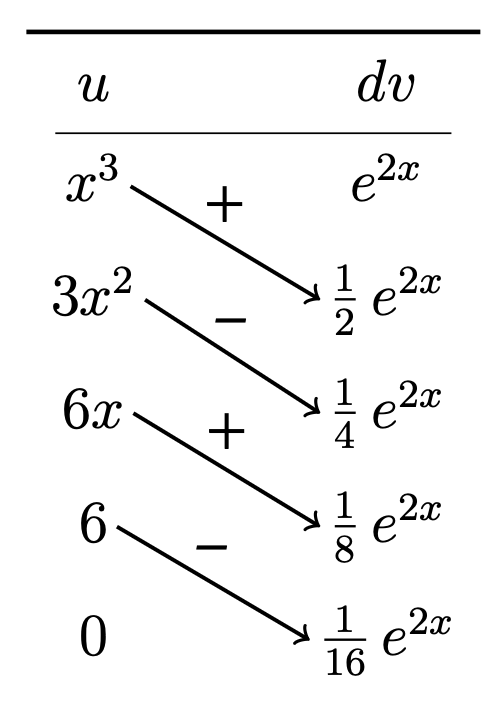
\includegraphics[width=0.19\textwidth]{images/tabular.png}
	\end{figure}
So that\dots
	\[
	\int x^3 e^{2x} \;dx= \dfrac{1}{2}\, x^3 e^{2x} - \dfrac{3}{4}\, x^2 e^{2x} + \dfrac{6}{8}\, x e^{2x} - \dfrac{6}{16} e^{2x} + C
	\]

\item Be able to compute integration-by-parts where one has to `loop back' to the original integral, i.e. `looping integrals'. 

\item Be able to recognize when an integral may be a `looping integral', e.g. $\ds\int e^x \sin x \;dx$ or $\ds\int \sin(2x) \cos x \;dx$, etc. This occurs most often when the integrand is of the form $\text{exponential} \cdot \text{trig}$ or $\text{trig} \cdot \text{trig}$ (but the trig functions have non-matching arguments).

\item Be able to use tabular integration to compute `looping' integrals, e.g. $\ds\int e^x \cos(2x) \;dx$
	\begin{figure}[H]
	\centering
	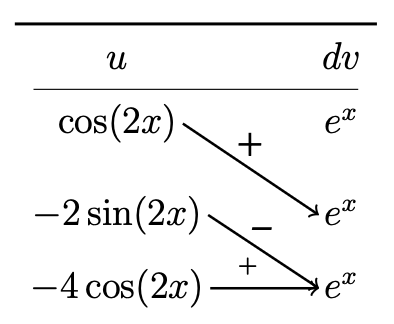
\includegraphics[width=0.22\textwidth]{images/looping.png}
	\end{figure}
So that\dots
	\[
	\begin{gathered}
	\int e^{x} \cos(2x) \;dx= e^x \cos(2x) + 2 e^x \sin(2x) - \int 4 e^x \cos(2x) \;dx \\[0.3cm]
	\int e^{x} \cos(2x) \;dx= e^x \cos(2x) + 2 e^x \sin(2x) - 4 \int e^x \cos(2x) \;dx \\[0.3cm]
	5 \int e^{x} \cos(2x) \;dx= e^x \cos(2x) + 2 e^x \sin(2x) + C \\[0.3cm]
	\int e^{x} \cos(2x) \;dx= \dfrac{1}{5} \left( e^x \cos(2x) + 2 e^x \sin(2x) \right) + C
	\end{gathered}
	\]

\item Be able to distinguish between integrals which require $u$-substitution, integration-by-parts, or both. 

\item Be able to compute some `shifting integrals' instead by integration-by-parts, e.g. $\ds\int x(2x + 1)^5 \;dx$ or $\ds\int \dfrac{x}{\sqrt{4x + 5}} \;dx$.
\end{itemize}

% 08/21, Thursday: Integration-by-Parts
\newpage
\section*{08/21, Thursday: Integration-by-Parts\label{08-21}}

\begin{itemize}
\item Know the integration-by-parts formula: $\ds\int u \;dv= uv - \int v \;du$, or in the case of a definite integral $\ds\int_a^b u \;dv= uv \bigg|_a^b - \int_a^b v \;du$.

\item Recall that the integration-by-parts formula comes from manipulating the product rule for derivatives, so it is a kind of `reverse product rule'.

\item Be able to use integration-by-parts to compute integrals. 

\item Recognize integrals where integration-by-parts may be appropriate, e.g. $\int x^2 \ln x \;dx$, $\ds\int x^2 e^{3x} \;dx$, $\ds\int \arctan x \;dx$, $\ds\int \ln x \;dx$, $\ds\int e^x \sin x \;dx$, etc. 

\item Be able to use LIATE and the `box method' to perform integration by parts, where\dots
	\begin{table}[H]
	\centering
	\begin{tabular}{rl}
	L: & Logarithms \\
	I: & Inverse Trig \\
	A: & Algebraic \\
	T: & Trigonometric \\
	E: & Exponential
	\end{tabular}
	\end{table}
One then creates a box and fills it in:
	\begin{figure}[H]
	\centering
	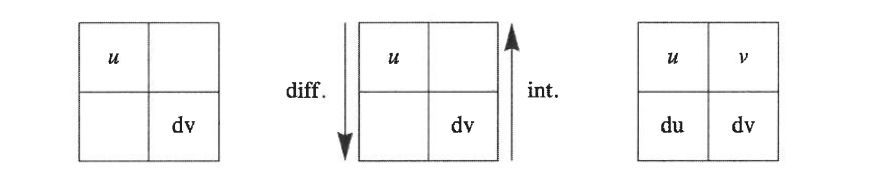
\includegraphics[width=0.80\textwidth]{images/box.png}
	\end{figure}
and then applies the `rule of 7':
	\begin{figure}[H]
	\centering
	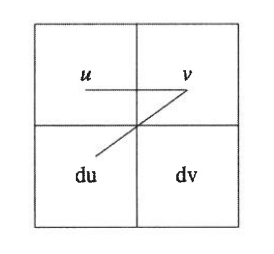
\includegraphics[width=0.20\textwidth]{images/7.png}
	\end{figure}
One can then write down $\ds uv - \int v \;du$. 

\item Know that the idea of integration-by-parts (by LIATE or otherwise) is to choose $dv$ to be the `hardest' part of the integrand that one can actually integrate, i.e. to simplify the integral by `integrating out' the hardest part possible and hope the resulting integral will be simpler. 

\item Know that LIATE can fail but often `overgrabs', i.e. $\ds\int x^3 e^{x^2} \;dx$ and how to fix it in this case. But also know that LIATE can fail completely, i.e. $\ds\int \dfrac{x e^x}{(1 + x)^2} \;dx$, and know how to `fix' $u$ and $dv$ in the case where LIATE totally fails. 

\item Be able to compute integrals where one first has to make a $u$-substitution before applying integration-by-parts, e.g. $\ds\int e^{\sqrt{x}} \;dx$ ($u= \sqrt{x}$), $\ds\int \sin(\sqrt[3]{x}) \;dx$ ($u= \sqrt[3]{x}$), etc.

\item Know that sometimes one has to perform integration-by-parts more than once to compute a given integral, e.g. $\ds\int x^2 e^x \;dx$ or $\ds\int x^3 \cos x \;dx$, or that some integration-by-parts integrals can `loop back' on themselves, e.g. $\ds\int e^x \sin x \;dx$ or $\ds\int \sin(2x) \cos(3x) \;dx$. 

\item Know that the integrals $\ds\int e^{x^2} \;dx$, $\ds\int \sin(x^2) \;dx$, and $\ds\int \cos(x^2) \;dx$ are all `impossible'. 
\end{itemize}

% 08/19, Tuesday: $u$-Substitution Review
\newpage
\section*{08/19, Tuesday: $u$-Substitution Review\label{08-19}}

\begin{itemize}
\item Know that $\ds\int_a^b f(x) \;dx$ represents the net area `under the curve' $f(x)$ between $x= a$ and $x= b$, i.e. the net directed area between $f(x)$ and the $x$-axis between $x= a$ and $x= b$---area under the $x$-axis counting as negative.

\item Know that if $\ds\int f(x) \;dx= F(x)$, then $\ds\int_a^b f(x) \;dx$ computes the net change in $F(x)$ between $x= a$ and $x= b$, i.e. $\ds F(b) - F(a)= \int_a^b f(x) \;dx$.

\item Memorize the `elementary' integrals:
	\begin{2itemize}
	\item $\ds\int \# \;dx= \#x + C$
	\item $\ds\int x^n \;dx= \dfrac{x^{n+1}}{n+1} + C, n \neq -1$
	\item $\ds\int \dfrac{1}{x} \;dx= \ln|x| + C$
	\item $\ds\int \sin x \;dx= -\cos x + C$
	\item $\ds\int \cos x \;dx= \sin x + C$
	\item $\ds\int \tan x \;dx= \ln|\sec x| + C$
	\item $\ds\int \sec x \;dx= \ln|\sec x + \tan x| + C$
	\item $\ds\int \csc x \;dx= \ln|\csc x - \cot x| + C$
	\item $\ds\int \cot x \;dx= \ln|\sin x| + C$
	\item $\ds\int \sec^2 x \;dx= \tan x + C$
	\item $\ds\int \sec x \tan x \;dx= \sec x + C$
	\item $\ds\int \csc^2 x \;dx= -\cot x + C$
	\item $\ds\int e^x \;dx= e^x + C$
	\item $\ds\int a^x \;dx= \dfrac{a^x}{\ln a} + C$
	\item $\ds\int \ln x \;dx= x \ln x - x + C$
	\item $\ds\int \log_b x \;dx= \dfrac{x \log_b x - x}{\ln b} + C$
	\item $\ds\int \dfrac{1}{1 + x^2} \;dx= \arctan x + C$
	\item $\ds\int \dfrac{1}{\sqrt{1 - x^2}} \;dx= \arcsin x + C$
	\end{2itemize}

\item Know when $u$-substitution might be appropriate: when one has a function one can integrate but is `off' by a factor whose derivative (up to a multiple) is in the integrand. For example, $\ds\int x e^{x^2} \;dx$. Here we know how to integrate $e^x$ but is `off' by $x^2$, whose derivative $2x$ can be found (up to a multiple) in the integrand, i.e. the $x$.

\item Know how to use $u$-substitution with both definite and indefinite integrals, e.g. $\ds\int \dfrac{\sin(\ln x)}{x} \;dx$ and $\ds\int_1^4 \dfrac{e^{\sqrt{x}}}{\sqrt{x}} \;dx$.

\item Be able to perform linear $u$-substitution in your head, i.e. one should be able to compute integrals `like' $\ds\int e^{3x} \;dx$, $\ds\int \sin\left( \tfrac{x}{2} \right) \;dx$, $\ds\int (2x - 1)^5 \;dx$, etc. in one's head. 

\item Remember to always change your bounds when performing $u$-substitution with a definite integral!

\item Recognize the special case of $u$-substitution of `shifting' integrals, where one needs to solve for $x$ in $u= \cdots$, e.g. $\ds\int \dfrac{x}{x + 3} \;dx$, $\ds\int x \sqrt{x - 2} \;dx$, $\ds\int 4x(x + 3)^{10} \;dx$, etc. 
\end{itemize}

\end{document}